\documentclass{article}
\usepackage{hyperref}
\usepackage{svg}
\usepackage{caption}
\usepackage{subcaption}
\usepackage{graphicx}
\usepackage{float}
\usepackage[utf8]{inputenc}\usepackage[
backend=biber,
style=apa
]{biblatex}
\addbibresource{bib.bib}

\title{VSN - Koalarization in PyTorch}
\author{Casper Smet - 1740426}
\date{2022/04/10}

\begin{document}

\maketitle

\section{Introduction}
    
    The colourisation of grey-scale images is useful in many different domains, states \cite{deepkoal2017}. With perhaps the most notable example the re-mastering of historical photographs.
    
    In the paper "Deep Koalarization: Image Colorization using CNNs and Inception-Resnet-v2", the authors claim that extracting high level features\footnote{e.g. recognising  plants or water} can improve the colourisation results.
    Their method uses CIELAB colour space (\cite{Luo2014}). CIELAB contains three channels, with channel L(uminescence) being a kind of grey-scale of the image, and A*B* being colour channels. \cite{deepkoal2017} attempts to predict the latter in their experiment using the prior.
    
    \cite{deepkoal2017}'s results were impressive. However, they made one critical error. They use the L-channel from the original, in-colour, image. Ergo, their model uses some apriori that it should not have.
    
    In this paper, we replicate the experiment with the Luminescence channel taken from a grey-scale image. We hypothesise that the results using grey-scaled images will be similar in quality to the original method's results, as the differences in the luminescence channels of the two methods are, to human vision, small.

\newpage
\tableofcontents
\newpage

\section{Background} \label{background}
    % Talk about the Koalarization paper, Inception-Resnet-v2, PyTorch, TIMM, the ImageNet dataset.
    
    In this section we give some background on this replication study. Namely, the structure of \cite{deepkoal2017} network and their experiment, including a description of Inception-ResNet-v2. Furthermore, we describe the modules and frameworks used in this experiment. Finally, we describe the ImageNet project, who's data was used in both this and \cite{deepkoal2017}'s experiment.
    
    % Some background is required in order to understand this paper
    % In this section, we explain the structure of the original paper's model
    % What inception-Resnet-v2 is
    % The machine learning framework we used, including the external library used for some of this implementation's features.
    % And finally, this project's datasource, the ImagenNet project.
    \subsection{Original paper}
    \subsubsection{Network architecture}
    % \cite uses a combination of Convolutional Neural Networks and Inception-ResNet-v2 in order to estimate A*B* colour channels.
    % The network is divided into four components
    % feature extractor, encoder, fusion, decoder 
    % The latter three only subsisting of convolutional neural networks and upsampling
    % the fusion layer combines the extracted features from the feature extractor with the features extracted by the encoder before feeding this into the decoder.
        \cite{deepkoal2017}'s Colorization network is built up from a combination of Convolutional Neural Networks\footnote{Hereafter referred to as CNNs} and Inception-ResNet-v2. Its input being the L* channel, and its output being the A*B* colour channels from the CIELAB standard.
        
        The network is divided into four components:
        \begin{enumerate}
            \item Feature extractor\footnote{Inception-ResNet-v2}
            \item Encoder
            \item Fusion
            \item Decoder
        \end{enumerate}
        With the latter three subsisting only of CNNs and upsampling layers. The Encoder and Feature extractor components both take the L* channel as input. The Fusion component then combines the extracted high-level features from the Feature Extractor with the mid-level features from the Encoder. It then convolves over the embedding, and passes the result onto the Decoder component. The Decoder component convolves over this and then returns the A*B* colour channels.
        
    \subsubsection{Experiment}
        They trained this network using mean squared error as the loss criterion. This is, however, not how \cite{deepkoal2017} judged their model's results. Instead, the original paper tested their model's performance through a user study.
        
        They present the user with a set of twelve images, nine recoloured images and three original images. Next, they asked to choose which images were fake or real.
        
        According to their study, 45.87\% of users miss-classified recoloured images as real. It is important to mention that the recoloured images used were selected from their best results.
    
    % The original paper tested their model's performance through a user study. They presented the user with a set of carefully selected recoloured images, and original images and asked them to select whether they were fake or real.
    
    % They computed that 45.87% of users miss-classified recoloured images as "real". Noting however, that the recoloured images were selected from their best results.   
        
    \subsection{Inception-ResNet-v2} \label{resnet}
        Inception-ResNet-v2 is a neural network architecture for multi-label image classification. It is one of three architectures introduced in \cite{szegedy2017inception}. Inception-ResNet-v2 is a combination of the Inception architecture and "Residual Connections"\footnote{i.e. ResNet}(\cite{DeepRes}).
        
        Inception-ResNet-v2 is trained on the ImageNet database (\cite{deng2009imagenet}). Therefore, it classifies 1000 different classes.
        
        At the time of its release, it had the highest Top-5 accuracy on Papers with Code's\footnote{A aggregator of scientific papers with source code. Also offers leaderboards for different challenges} Image Classification on ImageNet\footnote{\href{https://paperswithcode.com/sota/image-classification-on-imagenet?metric=Top\%205\%20Accuracy}{paperswithcode.com/sota/image-classification-on-imagenet}} challenge with a score of 95.1\%. Shortly after it was supplanted by ResNet-200, with a score of 95.2\%. Today, on 2022/03/30, Inception-ResNet-v2 is the 102nd best performing model on the Image Classification on ImageNet challenge.
        
        In this project, a pretrained implementation of Inception-ResNet-v2 was used. See \ref{torch} for more information about this implementation.
        % Inception resnet v2 is an architecture for multi-label image classification.
        % inc-res was one of three architectures introduced in paper
        % The pre-trained version was trained on the imagenet dataset (ref)
        % The implementation/weight training/ was done by TIMM

    
    \subsection{Pytorch and the Torch-Image-Models library (TIMM)} \label{torch}
        The original paper's implementation was made with the deep learning framework Keras-Tensorflow (\cite{chollet2015keras}).
        
        However, for the sake of variety, this implementation was done in PyTorch (\cite{NEURIPS2019_9015}) instead. Like Keras-Tensorflow, PyTorch is a high performance deep learning framework.
        
        Unlike Keras-Tensorflow, PyTorch does not come with an implementation of Inception-ResNet-v2. Torch-Image-Models\footnote{Hereafter referred to as TIMM} by \cite{rw2019timm}'s implementation is used instead.
        
        TIMM offers authentic implementations of various architectures in PyTorch. For some of the architectures, including Inception-ResNet-v2, pretrained models are also available. 
        % This implementation is done in PyTroch instead of Tensorflow/Keras. 
        % Pytorch, like Tensorflow, is a high performance deep learning framework
        % A popular external library for Pytorch is Torch-Image-Module, or TIMM. 
        % TIMM contains implementations for image architectures, often also offering pre-trained netwerks
    
    \subsection{ImageNet} \label{imagenet}
    % The imagenet project is a ongoing research effort for collecting and labelling iage data for object recognition models. ImageNet (dataset) is labelled based on the WordNet synset.
    % There are a number of iterations of the ImageNet dataset
    % The original paper used the 2011 iteration of ImageNet.
    % The iterations from 2021 and later are combined into one large dataset.
    % This iteration is seemingly no longer available. 
        The ImageNet project is a ongoing research effort for collecting and labelling image data for object recognition models. ImageNet (the database) uses labelling based on the WordNet lexical dataset (\cite{Fellbaum1998}).
        
        The ImageNet database is updated every few years. With the years 2012-2018 being combined into one larger database. \cite{deepkoal2017} uses the 2011 iteration of ImageNet. As this iteration is no longer available, the next iteration is used instead. That being the 2012-2018 iteration.

\section{Methodology}
    
    \subsection{Data collection} \label{data_col}
        % As mentioned above, data is collected from the ImageNet. We use a different version from the original authors (2012 vs 2011) due to availability problems.
        % Sourced from kaggle
        % ImageNet's validation set is ensured to balanced
        % We take a small subset of 10K images, and break this up (9:1) as a train and validationset.
        % This is considerably smaller than the original authors' dataset (60K) images. This is due to hardware constraints.
        % We assume the balance transfers to this subset
        % ImageNet labels are unused, as the images are both input and target.
        As mentioned in \ref{imagenet}, the data is collected from the ImageNet project. A different iteration of the database from the original authors is used for this project due to availability problems.
        
        This experiment uses the subset of the ImageNet database sourced from \href{https://www.kaggle.com/c/imagenet-object-localization-challenge/overview/description}{Kaggle}\footnote{\href{https://www.kaggle.com/c/imagenet-object-localization-challenge/overview/description}{kaggle.com/c/imagenet-object-localization-challenge}}
        
        The validation set is ensured to be balanced by ImageNet. Ergo, it is assumed that a randomised subset of this data will be approximately as balanced.
        
        Due to hardware constraints, the subset of images used for this experiment is smaller than that of the original authors. The original authors used 60 thousand images, this experiment only uses 45 thousand. The ratio of train-validation images is kept at 8:1, only slightly differing from the original's ratio of 9:1.
        
        The labels supplied by ImageNet are left unused, as the images are both input and target.
        
    
    \subsection{Replicating Koalarization}
        In order to replicate the Koalarization paper, a Python Module was developed. This module can be found at \href{https://github.com/Casper-Smet/koalarization\_torch}{github.com/Casper-Smet/koalarization\_torch}. The module can be installed, and binaries are provided for every release. 
        
        As described in \ref{torch}, this implementation was written using PyTorch. The behaviour of the original of the original implementation is replicated as closely as possible. In order to accomplish this, some modules must be implemented independently.
        
        For example, the Conv2D layer in PyTorch does not support both 'same' type padding and the use of stride. Nor is there a function for resizing an image with padding, or converting an image CIELAB to SRGB and vice versa. These features were either implemented independently, or imported from TIMM.
        % Python module
        % Written in PyTorch
        % Tensorflow behaviour is replicated as closely as possible, so some things must be implemented independently
        % I.e, Conv2d with stride and same padding, padding and crop, cielab to rgb, etc
        
    \subsection{Luminescence channel}  \label{lum}
        Like mentioned in the introduction, unlike the original implementation this implementation takes the L* channel from a grey-scaled version of the original image. The extraction of the L* channel takes place in the dataloader module. Ergo, altering the code to reflect the original paper better would be trivial.
        

    % Original paper used a rgb->grayscale version of the image for the resnet, but the luminescence component of the image for the encoder. While the luminescene component of the image. The original paper doesn't mention much about this process.

\section{Experiments} \label{experiments}

    % Train model for n epochs on k thousand images
    % Copy the parameters from the original experiment, now with images recoloured by this implementation of Koalarization
    % Select subset of images where model performed well
    % Make a form where the user receives 12 random images
    % 9 recoloured
    % 3 real
    % Ask user to select which images are real/fake
    % Hope to receive similar amount of responses (around 41)
    % Collect results
    % If 45% +- 5% of users miss-classify recoloured as real, experiment is a succes
    % Otherwise, ???
    In order to validate \cite{deepkoal2017}'s experiment, we intend to repeat it.
    
    Therefore, we will train a model on our dataset copying the original experiment's parameters. Next, the trained model is used to recolour all images in the validation set. From these recoloured images, the most convincing ones are selected.
    
    Using these recoloured images, a user study is created. The user is presented with nine recoloured images and three original images. Next, the user is asked which images are real and which are fake. The rate at which users miss-classify the fake images as real is called the realness perception.
    
    The original paper collected about 41 responses. This paper collected 60 responses.
    
    % Because, due to hardware and time constraints, it is not possible to train the model as long as the original paper, the testing criterion will be defined more leniently. The target realness perception will be 5\% lower than that of the original paper.
    
    % Ergo, if greater or equal to 40.87\% of users miss-classify the recoloured images as real, the original method is considered validated.
    
    We define the following hypothesis:
    \begin{quote}
        $H_{0}: r_{1} = r_{2}$
    \end{quote}
    Where $H_{0}$ is the null hypothesis, $r_{1}$ is the realness perception of the original experiment, and $r_{2}$ is the realness perception of this experiment.
    
    This hypothesis will be tested using a two-sided t-test\footnote{See \href{https://docs.scipy.org/doc/scipy/reference/generated/scipy.stats.ttest\_ind\_from\_stats.html\#r24a95fcea38c-1}{docs.scipy.org/doc/scipy/reference/generated/scipy.stats.ttest\_ind\_from\_stats.html}}.
    
    If the p-value is found to be lower than the alpha value of 0.05, the $H_{0}$ is to be rejected. Otherwise, this test confirms \cite{deepkoal2017}'s experiment.
    
    
    
    \subsection{Training}
        As mentioned in \ref{data_col}, the model is trained on 40 thousand images, with five thousand images being held out for use as validation data. All images colourised in this report are from the validation set unless specified otherwise. 
        
        All images are padded to be square and resized to 244x244. The resultant images then have their A*B* colour channels extracted and simultaneously are converted to grey-scale and have their luminescence channel extracted. The former serving as the model's target, and the latter as it's input. These values are also normalised to [-0.5, 0.5]. 
        
        Just like the original experiment, the network is trained using the ADAM optimiser (\cite{ADAM}) with a learning rate of 0.001. The loss function is Mean Squared Error, or MSE.
        
        After every 100 batches, the running loss and some colourised images from the train set are uploaded to Tensorboard to keep track of progress. At the end of each epoch, the running loss is calculated over the validation set. This, along with some colourised images from the validation set are uploaded to Tensorboard.
        
        By default, the Tensorboard logs can be found in \texttt{./log/koala/*DATE*}.
        
        \begin{figure}
            \label{fig:loss}
            \begin{subfigure}[b]{0.5\textwidth}
                \centering
                % \includesvg[width=\textwidth]{img/train_loss.svg}
                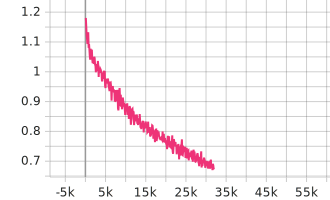
\includegraphics[width=\textwidth]{img/train_loss.png}
                \caption{Per 100 train batches on train data, running loss}
                \label{fig:train_loss}
            \end{subfigure}
            \hfill 
            \begin{subfigure}[b]{0.45\textwidth}
                \centering
                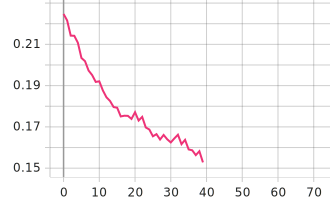
\includegraphics[width=\textwidth]{img/val_loss.png}
                \caption{Entire validation dataset per train epoch}
                \label{fig:val_loss}
            \end{subfigure}
            \caption{MSE-loss graphs during training. \textit{y}-axis equals loss}
        \end{figure}
        
        The model was trained for 40 epochs on a laptop\footnote{Asus ROG Strix GL702VS-GC198T} with a NVIDIA GeForce GTX 1070, 16 GB of RAM. Using 8 workers for loading in the data, and a batch size of 50, this took approximately 13 hours.
        
        Based on the angle of the loss curve in figures \ref{fig:train_loss} and, more importantly, \ref{fig:val_loss}, the model has not started over-fitting. Ergo, it might be worthwhile to train the model for a greater number of epochs
        
        The majority of these hyper-parameters can be changed using command line arguments. For user instructions, see \href{https://github.com/Casper-Smet/koalarization\_torch#train}{github.com/Casper-Smet/koalarization\_torch}.
    
    \subsection{Results}
        After training the model on the train subset, the trained model is used to recolour the validation subset. This was done using the evaluation script\footnote{See \href{https://github.com/Casper-Smet/koalarization\_torch/blob/main/koala/evaluate.py}{github.com/Casper-Smet/koalarization\_torch/blob/main/koala/evaluate.py} and the instructions in \href{https://github.com/Casper-Smet/koalarization\_torch}{the README.md}.}
        
        The resulting images appear highly similar to those of the original experiment. This includes the flaws described by \cite{deepkoal2017}. Some images have been recoloured near-photo-realistically. However, the majority of the images are recoloured with some glaring artefacts, which are usually spots or slashes of bronze-grey.
        % After training the model on the train set, the script "evaluate" is used on the validation set
        % To generate a set of recoloured images
        
        % The results appear highly similar to those of the original experiment, with similar flaws in the generated images.
        
        % Some images give near-photo-realistic results whn recoloured, most however are recoloured with glaring artefacts, usually spots or slashes of bronze-grey/
        \begin{figure}[H]
            \centering
            \includegraphics[width=\textwidth]{img/example.png}
            \caption{Comparisons between original (ground truth), grey-scaled and recoloured images.}
            \label{fig:recol1}
        \end{figure}
        
        In figure \ref{fig:recol1}, some of the most near-photo-realistic images are placed next to their grey-scale and ground truth versions. The first image is very realistic looking, yet clearly oversaturated in comparison to its ground truth. However, this is a rare phenomenon. Furthermore, the background is coloured using orange, just as the tiger. The generated image is clearly different from the original, yet still believable. 
        
        The latter images show clear undersaturation, which is by far the more common problem found in the generated images. Specifically, the foliage on rows 2 and 3 are clearly undersaturated in comparison to their ground truth. This falls inline with the original paper's results: the model seems conservative with its colour-use.
        
        Finally, the model does not seem to perform well on human subjects. At most, parts of the subject skin are coloured correctly. Mostly, it leaves the subjects skin grey. The image in the last row is, in the author's opinion, the best recoloured image with a human in it.
        
        While this problem is not mentioned explicitly in the original paper, it is apparent when looking at their generated images. See figure \ref{fig:origin}.
        
        \begin{figure}[H]
            \centering
            \includegraphics[width=\textwidth]{img/origin_paper_examp.jpg}
            \caption{Left colourised by \cite{deepkoal2017}, right ground truth. Adapted from \cite{deepkoal2017}.}
            \label{fig:origin}
        \end{figure}
        % see fig recol1 for examp of near-photo-realistic images. First image appears somewhat over-saturated. This being a rare phenomenon. and it coloured the background the same colours as the tiger
        
        % The latter images show clear under-saturation. Which is the more common problem 
        
        % Finally, model does not work well on human subjects
        
        
        \subsubsection{User study}
        The user study was done using the Google Forms platform\footnote{Though the form is now closed, it could be found at \href{https://forms.gle/mm8cPUM3ggne8E6dA}{forms.gle/mm8cPUM3ggne8E6dA}.}. The anwers were analysed using Pandas in a Jupyter Notebook\footnote{See \href{https://github.com/Casper-Smet/koalarization\_torch/blob/main/Userstudy.ipynb}{github.com/Casper-Smet/koalarization\_torch/blob/main/Userstudy.ipynb}}.
        % The results from the google form(footnote) were processed in (link to jupyter)
        % Below, see the 9 recoloured images shown to the user
        
        See figure \ref{fig:fool_res} for the nine recoloured images shown to the user, and how often the user was fooled by each individual image.
        
            \begin{figure}[H]
                \centering
                \includegraphics[width=\textwidth]{img/results_colourised.png}
                \caption{For each recoloured image we give the percentage of users that answered “Real” to the question Real or Fake? The images are sorted according to how often they fooled the user.}
                \label{fig:fool_res}
            \end{figure}
        
        The results were similar, yet slightly better, than the original experiment. Four out of the nine images fooled more than half of the users, just like the original experiment. Three other images fooled nearly half of the users, ranging between 40\% and 45\%. Lastly the last two images fooled slightly more than a quarter of the users. 
        
        The lower scoring end of the recoloured images score better than that of the original experiment's counterparts. 
        
        The original paper fooled the user 45.87\% of the time, with a standard deviation\footnote{Standard deviation of the scores [79.0, 69.1, 64.1, 54.3, 42.4, 35.9, 35.1, 17.9, 15.0]} of 22.36\%. This experiment outperformed in both, fooling the users 48.5\% of the time, with a standard deviation of 17.1\%.
        
        These values are further processed in the aforementioned Jupyter Notebook. The t-test yielded a p-value of 0.493. $0.493 > 0.05$, ergo, the null-hypothesis cannot be rejected. The slightly greater realness perception and smaller standard deviation are not statistically significant. 
        
        
        % Results were similar to the original papers, though slightly better. 
        % 4 out of nine images fooled more than half the users, just like original. Three fooled nearly half (40-45%), better than original and the last two about one quarter. 
        % Lowest result in this experiment scores higher (15.0 vs 26.7), highest scores slightly worse
            

\section{Conclusion}
    Despite this experiment's changes to how the luminescence channel was procured, we hypothesised that the results of this experiment would not differ significantly from \cite{deepkoal2017}. We believed this to be the case based on the fact that the L* channel is not visually distinguishable when extracted from grey-scale than when its from the coloured image.
    
    As expected, the results from this experiment are approximately equal to the original experiment. 
    This result validates \cite{deepkoal2017}'s experiment.
    
    This experiment also reconfirms the weaknesses of the Koalarization architecture. Namely, that this network is not performant in colourising low-level image components like human subjects or dogs. It also confirms that most resulting images are undersaturated.
    
    This experiment also adds value outside of its validation purposes. As this implementation was written in PyTorch, as opposed to the original's Tensorflow-Keras. Thus, diversifying the Koalarization architecture's user base. Furthermore, this implementation is well-documented and modular. Ergo, it is highly adaptable.
    
    \subsection{Future work} \label{future}
        Firstly, we believe it to be prudent to train this model on the greater ImageNet database. 45 thousand images may seem like a lot, but consider that the ImageNet database contains one thousand classes. In a perfectly balanced mono-label\footnote{As the ImageNet database is multi-label, it is hard to say how the classes are balanced. See \ref{imagenet}} dataset, that amount to only 45 images per class. 
        
        Training on a larger dataset within a realistic time-frame would require greater computational ability. Future research should make use of compute clusters instead of home hardware.
        
        Secondly, the effects of the feature extractor should be examined, possibly through an ablation study. It would be interesting to see how it affects the colourisation of images.
        
        Thirdly, as Inception-ResNet-V2 is quite old, it would be interesting to see how a newer more performant feature extractor would impact this architecture's performance. For example, Floirence-CoSwin-H (\cite{florence}), which is, at this time, the highest scoring model in Top-5 accuracy on the Image Classification on ImageNet challenge.
        
        Finally, it would be worth expanding the user study with a greater and more varied number of images, both recoloured and original. In its current state, all users were presented with the same 12 images, though in a random order. Increasing the number of images presented to the users, and randomising the images shown, may give a more objective view on realness perception.
    % As expected, the results from this experiment are approx equal to that of the original paper, if not slightly better
    % This means our hypothesis is correct
    % The model works with 

\section{Discussion} \label{disc}
    \subsection{Automation}
        The user study may give a false impression of this model's performance. This is because the cherry picked colourised images do not fully represent the whole of this model's performance.
        
        While the results of this study are good, it is worth noting that full automation is a use case for which this model is simply not good enough. The model's colouring is simply too inconsistent for this use case. 
        
        The model may, however, still be useful in manual colourisation efforts, as it could give a starting point from which people may continue recolouring an image. This might help speed up the labour intensive process of manual colourisation.

% User study with cherry picked results is only representative for performance in a scenario without full automation 
% Would still be useful in speeding up manual colourisation
    \subsection{Population sample}
        The population under which this form was spread is largely Technical Informatics and Artificial Intelligence students at Hogeschool Utrecht. These users, especially the latter, could be better equipped to find mistakes in colourisation efforts versus the average consumer. This can be attributed to their profession. 
    
    \subsection{Different metrics}
        While the user study is a clear way to judge the models performance in the eyes of its users, it is difficult to use as an objective metric. Ergo, it is also difficult to compare different colourisation models in performance with this metric.
        
        Comparing this implementation with the \cite{deepkoal2017}'s implementation can be done by comparing the MSEloss on the validation set. To compare Deep Koalarization with other models, a standardised metric is in order.
        
        The metric currently used on the "Colorization on ImageNet val" leaderboard on PapersWithCode is Fréchet inception distance (\cite{heusel2017gans}), or FID in short. Future research might include this metric.
    
    \subsection{Colourising historic photographs}
        Real historic photographs are not always in perfect grey-scale. Often, these images are presented as sepia toned\footnote{See \href{https://en.wikipedia.org/wiki/Photographic\_print\_toning\#Sepia_toning}{en.wikipedia.org/wiki/Photographic\_print\_toning\#Sepia\_toning}}. Using grey-scaled versions of these images instead of their original sepia versions may cause data loss.
        % Form was spread among Technical Informatics and AI students / faculty. These users, esp the latter, might be better able to differentiate real from fake due to their profession.
    
    \subsection{Realness perception on original images}
        On interesting metric the original paper discarded, was the realness perception of the original images. See \ref{fig:originals_perc} for the scores of each individual image. The realness perception of the original images is 66.67\%.  The standard deviation in realness perception is 24.7\%.  In about one third of the cases, an original image is mistaken for a recoloured image. 
        
       However, with a sample size of original images this small, it is difficult to make any conclusions based on this information. This adds further need to expanding the user study as mentioned in \ref{future}.
       
       \begin{figure}[H]
           \centering
           \includegraphics[width=\textwidth]{img/originals_colourised.png}
           \caption{For each recoloured image we give the percentage of users that answered “Real” to the question Real or Fake? The images are sorted according to realness perception.}
           \label{fig:originals_perc}
       \end{figure}

% Higher score could also be attributed to the author's eye in choosing the recoloured images
  

\printbibliography{}

\appendix
\section{Appendix: Grading}
    \subsection{Implementing vision-algorithms (row 7)}
        For the purposes of this assignment, I implemented one algorithm. Namely: the Deep Koalarization image colourisation Neural network.
        
        The implementation is truthful to the original implementation, with the exception of one issue in the original implementation which I have remedied. This issue is technically not part of the architecture itself, but how data is prepared. See \ref{lum}.
        
        Furthermore, implementing this algorithm required a number of external libraries, namely:
        
        \begin{itemize}
            \item PyTorch, for basic machine learning functions
            \item Torchvision, for image manipulations
            \item PyTorch Image Models, for their implementation of Inception-ResNet-v2
            \item pytorch\_colors, for colour space manipulations, namely CIELAB
            \item Scikit Image, for colour space manipulations, namely CIELAB
        \end{itemize}
        
        These dependencies can be found in \href{https://github.com/Casper-Smet/koalarization\_torch/blob/main/setup.cfg}{github.com/Casper-Smet/koalarization\_torch/blob/main/setup.cfg} along with other utility dependencies used during data preparation, training, and validation.
        
        As PyTorch was not covered in class, using it required reading up on its literature. In addition to PyTorch, extra literature was required for implementing the CIELAB colour space, Inception-ResNet-v2 model, and the ImageNet database.
        
        Additionally, all code is documented. This includes class and function level docstrings. All docstrings follow the Google docstring standard. All code also fulfils the Flake8\footnote{See \href{https://flake8.pycqa.org/}{flake8.pycqa.org/}} standard, which is an expanded version of the Pep8 standard. The only exceptions to this rule are the Path variables, as they are often too long. Flake8 was configured locally in the \href{https://github.com/Casper-Smet/koalarization\_torch/blob/main/.flake8}{\texttt{.flake8}} configuration file.
        
        \begin{figure}[H]
            \centering
            \includegraphics[width=\textwidth]{img/flake8-results.jpg}
            \caption{flake8 linter ran against the code base}
            \label{fig:flake8}
        \end{figure}
        
        % Implemented one algorithm
        % The implementation is correct, and fixes a problem from the original paper (ref luminescence)
        % External libraries
        % All code is documented, and (except line length for path variables), fulfils the Flake8 standard (pep8 expansion)
        % The implementation requires pytorch and timm for the implementation of the network, skimage/pytorch_colors for colour space manipulations. The manipulating of the L* channel for Inc-RESNET required additional literature to implement
        
    \subsection{Use of literature (row 8)}
        % CIELAB, PyTorch image models, Inception-Resnet-v2, Hybrid networks
        In order to implement the Deep-Koalarization architecture, I had to read and process a number of different papers, articles and books. The most prominent of which I used as sources for this document\footnote{See bibliography}. Moreover, I documented some of these personally in chapter \ref{background}.
        
        Sources are also referenced in the code, both explicitly and implicitly. For example, see the \texttt{SquarePad} class in \href{https://github.com/Casper-Smet/koalarization\_torch/blob/main/koala/data.py#L36}{\texttt{koala/data.py}} for an explicit reference.
        
    \subsection{Planning (row 9)}
    
        My original planning was reasonably accurate, not including the period of illness. Furthermore, in case I underestimated the assignment I added optional tasks.
        
        Through week updates, changes in the planning on GitHub\footnote{See \href{https://github.com/Casper-Smet/koalarization_torch/blob/main/report/PLANNING.md}{github.com/Casper-Smet/koalarization\_torch/blob/main/report/PLANNING.md}}, and in person progress reports I kept the professor up to date.
        
        After a period of illness, I constructed a new planning via email that accounted for my two weeks of absence. This new planning, including deadline, was accepted.
        % Planning was reasonably accurate, not including period of illness
        % Through week updates, changes in the planning, in person meetings, kept prof up to date
    
    \subsection{GIT (row 10)}
        Both the professor and the Teaching Assistant were added to the GitHub repository. My commits were regular, despite the period of illness. See figure \ref{fig:com}.
        
        \begin{figure}[H]
            \centering
            \includegraphics[width=\textwidth]{img/commit-history.jpg}
            \caption{Git commit history for the git repository koalarization\_torch. Taken on 2022/04/07: 14:30}
            \label{fig:com}
        \end{figure}
        
        Furthermore, at the end of most workweeks, I created a release. These releases contain a binary in the form of a Python wheel\footnote{See \href{https://peps.python.org/pep-0427/}{peps.python.org/pep-0427/}}. The 1.0.0\footnote{See \href{https://github.com/Casper-Smet/koalarization\_torch/releases/tag/v1.0.0}{github.com/Casper-Smet/koalarization\_torch/releases/tag/v1.0.0}} release also contained a trained version of the Colorization network.
        % Teacher / TA added to GitHub
        % Commits were regular, releases were made, releases contained binaries for the module and later a trained model
    
    \subsection{Experiment (row 11)}
        The experiment, its parameters, and its results are well defined in \ref{experiments}. The experiments metrics, namely the MSE for training and the realness perception for validation are defined. These metrics are also interpreted using figures such as \ref{fig:val_loss} and \ref{fig:fool_res}.
        
        The uncertainty of realness perception is judged using a two-sided t-test. This ensures that the statistical significance of this experiment's result is taken into consideration when interpreting it.
        
        Finally, the author is critical of the metrics chosen to judge the Koalarization architecture. Most of this critique can be found in chapter \ref{disc}.
        % Experiment was well defined
        % Metrics: MSEloss for training, and more importantly realness perception/
        % These metrics are interpreted using figures
        % Uncertainty is handled by t-test
    
    \subsection{Report (row 12)}
        This report follows the structure found on Canvas. Furthermore, it is written for students who have followed the \textit{VSN} course at Hogeschool Utrecht. This includes the expectation of them knowing the basics of machine learning and CNNs. Materials that students are not likely to have encountered at this point were either explained or supplied with a source.
        
        All references are available in APA format.
        
        Moreover, the hypothesis made in the introduction, and its numerical derivative in \ref{experiments} are well formulated to be proven or disproved. The Conclusion and Discussion chapters also describe possible future work.
    
    \subsection{Experiment reproducibility (row 13)}
        All the scripts necessary for replicating this experiment can be found in the GitHub repository. Furthermore, it is clearly described where the data used in this experiment can be found. Finally, clear instructions are given on how to use these scripts, including (hyper)parameter selection. See the README.md for more information.
        
        Furthermore, Inception-ResNet-V2 can easily be replaced by another feature extractor without altering the code, as it is simply an argument the user can give when instantiating the Colorization network.
        
        Moreover, due to the nature of PyTorch as a machine learning framework, it would be easy to extend this code to ones own wishes. Be that subclassing the Colorization module or its submodules, writing your own dataset instance, or using a different optimiser. 
    


\end{document}
